\chapter{Load, Save, and the EDL}%
\label{cha:load_save_and_the_EDL}

There are many supported file formats that can be loaded and rendered to, that is to say, imported and exported. 
The format of the file affects what \CGG{} does with it.  
Some file formats are very slow to display on the timeline, especially video which is highly compressed.  
Drawing video thumbnails, picons, on the timeline can be very slow.  (You can disable picon drawing for these files with the \textit{draw media} toggle in the patchbay to speed up operations).

\section{EDL --- Edit Decision List}%
\label{sec:edl_edit_decision_list}

When \CGG{} saves a file, it saves the EDL, Edit Decision List, of the current project but does not save any media. 
Edit decision lists, more commonly referred to as the EDL, are generated by \CGG{} for storing projects.  
The EDL contains all the project settings and locations of every edit. 
Instead of media, the file contains pointers to the original media files on disk.  
EDL files are specific to \CGG{}.    

The EDL files generally have an extension of \texttt{.xml}.  
The purpose of the EDL is to separate the media from all of the editing operations so that the original media remains intact. 
When the \texttt{.xml} file is loaded, changes to the attributes of the current project are made based on the EDL\@. Edit decision lists are text files which means they can be edited in a text editor.  EDL and XML are used interchangeably.

\section{Supported File Formats}%
\label{sec:supported_file_formats}

There are basically 2 kinds of supported file formats, native and ffmpeg.  With the addition of ffmpeg, the majority of the supported file formats you will be using comes via this thirdparty package.  There are hundreds of ffmpeg file format and codec combinations. This set of possibilities includes qt (quicktime), avi (audio-video interleave),  mp4, mp3, mov, mpeg, m2ts, ts, wmv, mts, mpg, flv, mkv, webm, webp, ProRes and many more.

The other supported formats, referred to as \textit{native},  include the following:
AC3, 
Apple/SGI AIFF,
Sun/NeXT AU,
FLAC ,
Microsoft WAV,
Raw DV and PCM,
MPEG Audio and Video.

\paragraph{Still Images:}  JPEG/EXR/PNG/PPM/TGA/TIFF

\paragraph{MPEG Files:} 
What is an MPEG file?  A very common file format is MPEG because it works with many cameras and televisions.  Mpeg2 video, an elementary codec stream for mpeg files, is the most common format.  To read this format you need to decode the mpeg stream.  You can read and write mpeg natively.  Mpeg video encoding is done separately from mpeg audio encoding when using the native file format, meaning that 2 passes are required and then they have to be muxed together.  However, if using ffmpeg it is rendered in only 1 pass.  DVD uses MPEG as does NTSC and Pal.

\subsection{Working with Still Images}%
\label{sub:working_with_still_images}

Still images are played from 1 to any number of times, over and over; they have no duration. You can load still images on video tracks just like you do for any video file. When loaded on the track, use the down arrow on the timeline so you can see the single frame. To extend the length of the image, drag its boundaries just as you would do with regular video media. You can drag the boundaries of a still image as much as you want. Images in \CGG{} have the ability to be dragged to an infinite length. Alternatively, you can define the initial length of the loaded images. The parameter is set in the Images section of the \texttt{Settings $\rightarrow$ Preferences $\rightarrow$ Recording} window.

Unless your original material comes from a digital source using its best resolution (like a digital camera), the first thing you might have to do before you can use it is to somehow capture the assets into a usable digital medium. For old photos, paper maps, drawings or diagrams, you can scan them into a file format like PNG, TIF, TGA or JPG files by using a digital scanner.

Rendering a video to a single image causes the final image file to be overwritten for every timeline position. The rendered file is a single still image of the last frame of the video.

\subsection{Timelapse Sequence of Images, and Animation}%
\label{sub:timelaps_sequence_images_animation}

The next areas covered in this section are the following: 
\nameref{ssub:filelist_format} such as jpeglist and \nameref{ssub:image2ffmpeg}.

In order to be reasonably fast to use, you will most likely want to prepare them by creating a script and then load by utilizing this file generated script.

\subsubsection{Filelist format}%
\label{ssub:filelist_format}

An image sequence is a series of ordered still pictures; for example a bunch of camera shots, frames of an animated scene, or series of frame shots. These can be loaded as multiple files. For timelapse sequences, as the size of camera images increases to 70 megabytes and beyond, and more images can be stored on a memory stick, more cache, memory, and system resources (such as file descriptors) are used by \CGG{} to load the images when you use the \textit{concatenate tracks} or \textit{paste at insertion point} strategies.  It is very time consuming and resource consuming when each of the image files is loaded and concatenated as edits, and it also plays super poorly.  Here is an alternative to the usual \textit{load}.  This technique may also be useful for just a bunch of pictures.

File lists formats can be utilized in some way for the following list of types of \textit{Sequence files}  The first line of the sequence list file identifies the list codec.

%\vspace*{1ex}


\begin{center}
    \begin{tabular}{l l l l}
    PNGLIST = *.png	&	PPMLIST = *.ppm	&	TGALIST = *.tga	  &  TIFFLIST = *.tiff \\
    EXALIST = *.exa	&	CR2LIST = *.cr2	&	JPEGLIST = *.jpg	&    GIFLIST = *.gif
    \end{tabular}
\end{center}

%\vspace*{1ex} 
Using the example of jpeg’s, the jpeg list sequence file type is the easiest and fastest way to access a sequence of jpg images as a single asset.  First build a jpeglist sequence file and name it something like jpeglist.sh.  There is an example script of how to do this in the Auxiliary Programs section of the Appendix (\ref{sec:image_sequence_creation}).  Once the jpeglist.sh file is built you can then run it similar to this line:

\begin{lstlisting}[style=sh]
jpeglist.sh   /<path>/file.jpg   /<path>/DSC*.jpg
\end{lstlisting}

\vspace*{1ex} \noindent If <\texttt{path}> is the same on both outfile and infiles, then file.jpg is created in the same directory as infiles, the directory contains the entire asset, and the file list uses relative paths; otherwise the file list contains absolute paths.   Since this creates outfile list as a single asset, the memory demand and access time is much lower.  When you load the outfile in \CGG{}, you will need to set \textit{Try ffmpeg last} since ffmpeg does not work with jpeglist sequence files.

An example output file from running this script residing in the directory where \texttt{DSC*.jpg} files exist is shown below.

To use this, turn off ffmpeg probes first, and open \texttt{timelapse.jpg} using File $\rightarrow$ Load files.

\begin{lstlisting}[style=sh,caption={Example: timelapse.jpg},captionpos=t]
JPEGLIST
# First line is always JPEGLIST
# Frame rate:
29.970030
# Width:
6016
# Height:
4016
# List of image files follows
./DSC04948.jpg
./DSC04949.jpg
./DSC04950.jpg
./DSC04951.jpg
...(files in between)
./DSC04997.jpg
./DSC04998.jpg
\end{lstlisting}

\subsubsection{Image2ffmpeg}%
\label{ssub:image2ffmpeg}

Image2file format is an alternative method to open an image sequence via ffmpeg.  To do this, create 2 files in the same directory as the \texttt{DSC*.jpg} files named:  \texttt{DSC0\%04d.opts}, and \texttt{DSC0\%04d.jpg}. 
\texttt{DSC0\%04d.opts} should contain the following lines which have to be modified to fit your exact requirements for duration, start\_number, and frame\_rate.


\begin{lstlisting}[style=sh,caption={Example
    DSC0\%04d.opts},captionpos=t]
loglevel=verbose
threads=auto
format=image2
codec=mjpeg 
start_number=4948
frame_rate=29.97
duration=17.36
\end{lstlisting}

Example of the contents of the file \texttt{DSC0\%04d.jpg} would be just a single line as:  JPEG
In this case, make sure \textit{Try ffmpeg first} is enabled, and load \texttt{DSC0\%04d.jpg}.  
This will access the media using ffmpeg which is slower so be patient.

\subsection{Raw Image Format of Some Digital Cameras \& Probe Order}%
\label{sub:raw_image_format_digital_camera_probe_order}

\textit{Note: requires some expert knowledge.}  Raw digital camera images are a special kind of image file that \CGG{} can load. Dcraw, as used by \CGG{}, is Dave Coffin’s open-source computer program which reads many raw-image formats typically produced by many earlier and current digital cameras.  Currently over 700 of the types of cameras it recognizes are listed at:

\hspace{4em}	{\small \url{https://www.dechifro.org/dcraw/}}

For example, included are numerous models of Canon, Fuji, Kodak, Nikon, Olympus, and Panasonic as well as many others.  Because ffmpeg tries to load \textit{any and every} file if \textit{Try Ffmpeg first} is enabled, it will make an attempt to load Raw Camera files first before any other file driver gets the chance.  In addition, there is the possibility that dcraw could conflict with the standard TIFF format, since it might be seen as format type \textit{tiff-pipe}.  Therefore it is necessary to specifically enable CR2 and either move it to the top or disable \textit{FFMPEG\_Early} and enable \textit{FFMPEG\_late} in the \textit{Probe Order} as described in another section (\ref{sub:probe_order_loading_media} and \ref{sec:ffmpeg_early_probe_explanation}).  These changed settings will be retained across \CGG{} sessions in \texttt{.bcast5}.  Usage of Raw Camera mode generally requires more in depth knowledge of your specific camera.

The first screenshot in figure~\ref{fig:raw} as in \texttt{Settings $\rightarrow$ Preferences $\rightarrow$ Playback A} Tab, shows the default checked settings of \textit{Interpolate CR2 images} and \textit{White balance CR2 images} which display the raw images in a way that you expect.  However, you may want to uncheck them to ensure that no program manipulation has modified your images so that you can add plugins or make your own modifications.  Unchecked indicates that the images are as closest as possible to unadulterated raw.

The second screenshot showing CR2 for Raw Camera highlighed/enabled in the Preferences Probes’ screen.

The final screenshot showing the Resources Asset Info displaying the File format as Raw Camera.

\begin{figure}[htpb]
    \centering
    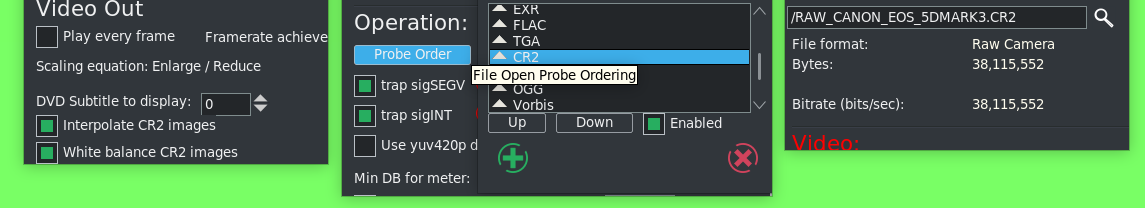
\includegraphics[width=0.95\linewidth]{raw.png}
    \caption{Screenshots for RAW images}
    \label{fig:raw}
\end{figure}

\section{Loading Files}%
\label{sec:loading_files}

All data that you work with in \CGG{} is acquired either by loading from disk or recording from a device. This section describes loading.  To bring up the Load window go to the File pulldown and choose Load Files  (figure~\ref{fig:load}).  Next \textit{Select files to load}, and click ok (the green checkmark) or \textit{Apply}. When you use the Apply button, the Load window remains active for easily loading more files later.  Depending on the setting of the Insertion Strategy list box, your file will be either loaded directly on the Program window or in the Resources Media window.  If the file is a still image, the project's attributes are not changed and the first frame of the track becomes the image. \CGG{} usually builds an index file if one does not already exist, in order to speed up drawing. You can edit and play the file while the index is being built.

\begin{figure}[htpb]
    \centering
    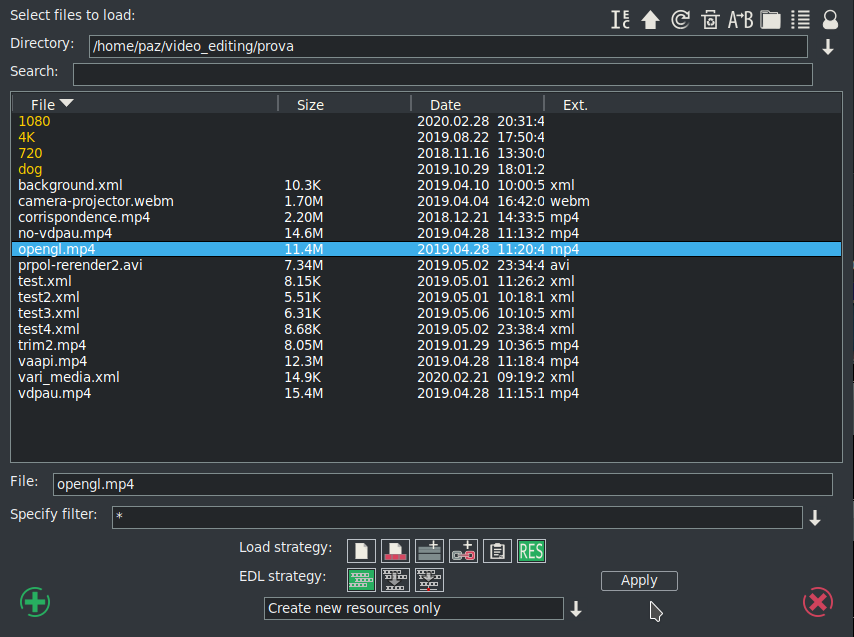
\includegraphics[width=0.9\linewidth]{load.png}
    \caption{Load file menu.  Note the green checkmark for OK and the middle Apply option}
    \label{fig:load}
\end{figure}

\vspace{1ex} \noindent To load a file, you will need to:

\begin{enumerate}
    \item set a directory path in the Directory input box
    \item choose a file or set of files by highlighting your selection
    \item select an insertion strategy for loading the file 
\end{enumerate}

\noindent Once you have completed making your choices and clicking OK or Apply, by default three things occur:

\begin{itemize}[noitemsep]
    \item The existing project is cleared from the screen.
    \item The project's attributes are changed to match the file's attributes.
    \item The new file's tracks are created in the timeline.
\end{itemize}

\noindent Let's now see in detail the options of loading files.

\begin{description}
    \item[Insertion Strategy] 
    \CGG{} lets you change what happens when you load a file.  In the Load dialog window go to the Insertion strategy box and select one of the options in the drop down menu. Each of these options loads the file a different way.
    
    \begin{description}
       \item [Replace current project:] all tracks in the current project are deleted and a set of new tracks are created to match the source file.  Project attributes are only changed when loading XML\@. If multiple files are selected for loading, \CGG{} adds a set of new tracks for each file. New resources are created in the Resources Window, replacing the current ones.
       \item [Replace current project and concatenate tracks: ] same as replace current project, except that if multiple files are selected, \CGG{} will concatenate the tracks of each file, inserting different source files in the same set of tracks, one after another, in alphanumeric order, starting at 0. New resources are created in the Resources Window, replacing the current ones.  Files go across the timeline.
    \end{description}
    For ffmpeg and mpeg files, when the Insertion strategy methodology in the \texttt{File $\rightarrow$ Load files} pulldown is chosen to be either \textit{Replace current project} or \textit{Replace current project and concatenate tracks}, the basic session format parameters are reinitialized to match new media.  This selects the default asset and determines its width, height, and video length, frame rate, calculates the colormodel, and assumes square pixels to make an intelligent guess about aspect ratio for video.  For audio, the sample rate, audio length, and channel count (mono, stereo, or 5.1) are reinitialized.  In addition the \textit{Track Size} will be computed and is reinitialized to match the new loaded media.  When using \textit{replace} type insertion strategy, the new asset list is the only media in use so that this update saves the user from immediately needing to change the session format to match the only possibility.
    \begin{description}
        \item[Append in new tracks:] the current project is not deleted and new tracks are created for the source, one set of tracks for each file. New resources are created in the Resources Window.  Files go down tracks.
        \item[Concatenate to existing tracks:]  the current project is not deleted and new files are concatenated to the existing armed tracks, inserted in the same set of tracks of the current project, one after another, in     alphanumeric order, starting at the end of the tracks. If the current project has more tracks than the source, the source file will be inserted in the first set of armed tracks. If no tracks are armed, no files will be inserted. New resources are created in the Resources Window.
        \item[Paste at insertion point:] the file is pasted into the timeline at the insertion point, on the first set of armed tracks.  If multiple files are selected for loading, they will be inserted on the same set of tracks, one after the other. New resources are created in the Resources Window.
        \item[Create new resources only:] the timeline is unchanged and new resources are created in the Resources Window only.
        \item[Nest sequence:] nested assets are added to the timeline by using the Nest sequence insertion strategy.
        The file will be pasted into the timeline over the current selection or at the insertion point. A nested sequence is media that had already been saved as an EDL earlier.  Nesting is described more fully in section \ref{sub:nesting}.
    \end{description}
    The insertion strategy is a recurring option in many of \CGG{}'s functions. In each place the options do the same thing. If you load files by passing command line arguments to \CGG{}, the files are loaded with \textit{Replace current project} by default.
    \item[Loading Multiple Files] In the Load dialog go to the list of files. Selecting files utilizes the motif style selection method.
    \begin{enumerate} [noitemsep]
        \item Select a single file by highlighting.
        \item Select multiple files by moving to another file and select it while holding down Ctrl. This selects
        one additional file.
        \item Or move to another file and select it while holding down Shift. This selects every intervening file.
    \end{enumerate}
This behavior is available in most listboxes.   It is an especially useful method when used with \textit{Concatenate to existing tracks} insertion strategy to create an images slideshow or a song playlist.
    \item[Loading files from the command prompt] Another way to load files is to pass the filenames as arguments on the command line.  This starts the program with all the arguments loaded and creates new tracks for every file.  For example:
    
    \texttt{\{your\_cinelerra\_program\_path\} video1.mp4 video2.mp4}
    \item[Finding Files by Extension, Sub-list, or with Search] If there are too many files in your media directory, it can be difficult to find the file you want. For this reason, the Load window allows you to filter which files are displayed in the list box by extension name. Click the dropdown box on the right side of the \textit{Specify filter} list box below the file name text box, and select the file extension of your media (for example: mp4, mov, mp3, avi, jpg, etc). The file list now shows only files with the selected extension.  Perhaps even easier is to use the Search box on the top underneath the \textit{Select files to load} listbox.  Here you can keyin a character or string to look for. \\
    You can also get a sub-list of potential files to choose from. For example, you know that the file you are looking for begins with the capital letter "C". If you keyin "C" into the selection box immediately below the list of files, and then click the left mouse button, a sub-list of files beginning with the "C" shows up under the selection box. Clicking the right mouse button cancels this sub-list.
    \item[Loading the backup] There is one special XML file on disk at all times. 

        After every editing operation, \CGG{} saves the current project to a backup in  \texttt{\$HOME/.bcast/backup.xml}. 
        In the event of a crash, the first thing you should do after restarting \CGG{} is select \texttt{File $\rightarrow$ Load backup} in order to load the backup. 
        This will start \CGG{} at the point in your editing operations directly before the program crashed. 
        It is important after a crash to restart \CGG{} without performing any editing operations as you will overwrite the backup. 
        Note that the backup.xml file is always a single file which means that when you are working with two instances of \CGG{} open at the same time, they use the same backup file. 
        In this case, the last operation made in whatever instance will overwrite the backup.
\end{description}

\subsection{Sort within Sort in File Load Dialog}%
\label{sub:sort_within_sort_file_load_dialog}

When you use the File pulldown to load files, you can do a sort within a sort when you click on the labeled header box (figure~\ref{fig:load-sort}).  This is useful, for example, when you want to find the smallest file for a specific extension.   In the screenshots below, the first illustrates the default \textit{File} sorted alphabetically; the second shows the \textit{Size} is now sorted; the third shows how after sorting on Size, you sort on Ext.  The size sort is maintained within the extension sort so that \textit{c.d} comes before \textit{a.d} in the File header box because the size is smaller.

\begin{figure}[htpb]
    \centering
    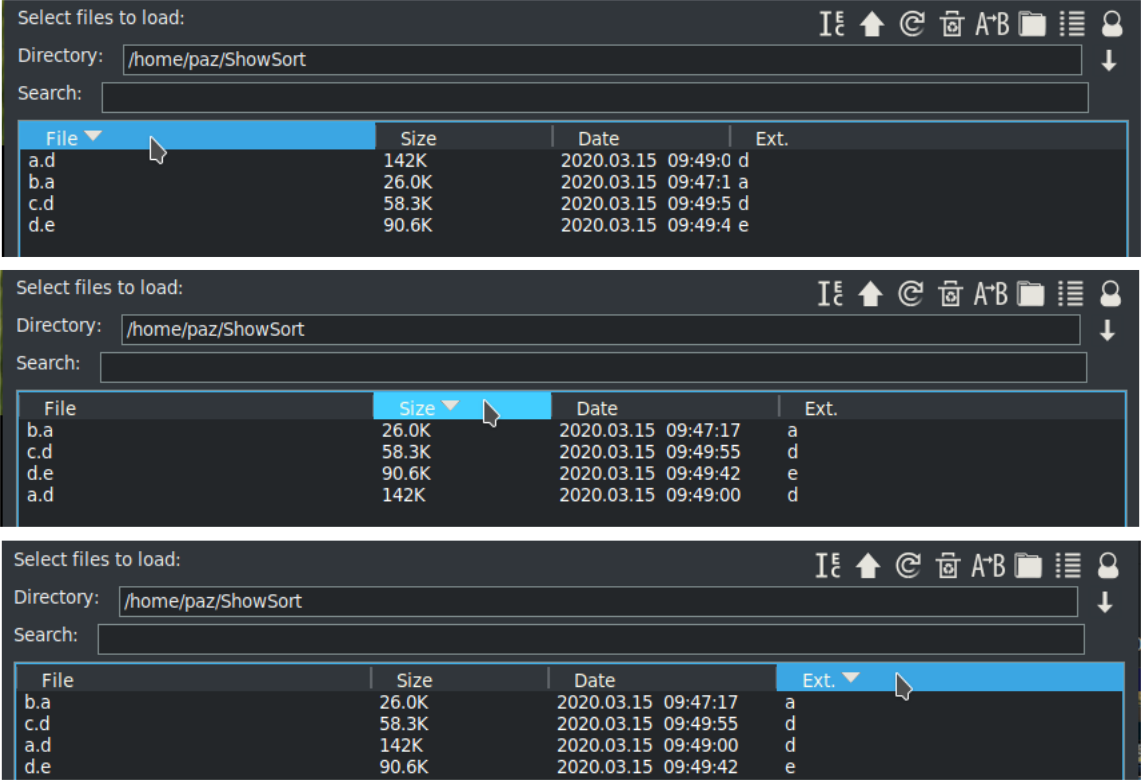
\includegraphics[width=1.0\linewidth]{load-sort.png}
    \caption{Load - Sort by File name, sort by file Size, and within Extension after a previous Size sort}
    \label{fig:load-sort}
\end{figure}

\subsection{Size Numeric Format Displayed in File Load}%
\label{sub:size_numeric_format_displayed_file_load}

There are several icon buttons at the top on the right hand side of the Load window.  Each has a tooltip to explain what it is for.  You can see these in the previous figure.  One is for File size format.  There are 4 numerical representation variations for reporting the file size in the \texttt{File $\rightarrow$ Load} pulldown.    You can see the options in the Load window to the right of the top line that read \textit{Select files to loads} (figure~\ref{fig:load-size}):

\begin{description}
    \item[0] this is the default and current behavior and shows bytes the same as the \textit{ls -l} command.
    \item[SI] 3 significant digits suffixed by lower case k,m,g,t,b for representing magnitudes in $10^3$ (1000)
    \item[Ic$^{E}$] 3 significant digits followed by upper case characters for representing magnitudes in $2^{10}$ (1024)
    \item[0,] like the exact default byte representation but with comma separators for easy reading.  Periods can
    not be used as separators due to locale conflict with ffmpeg coding.
\end{description}

\begin{figure}[htpb]
    \centering
    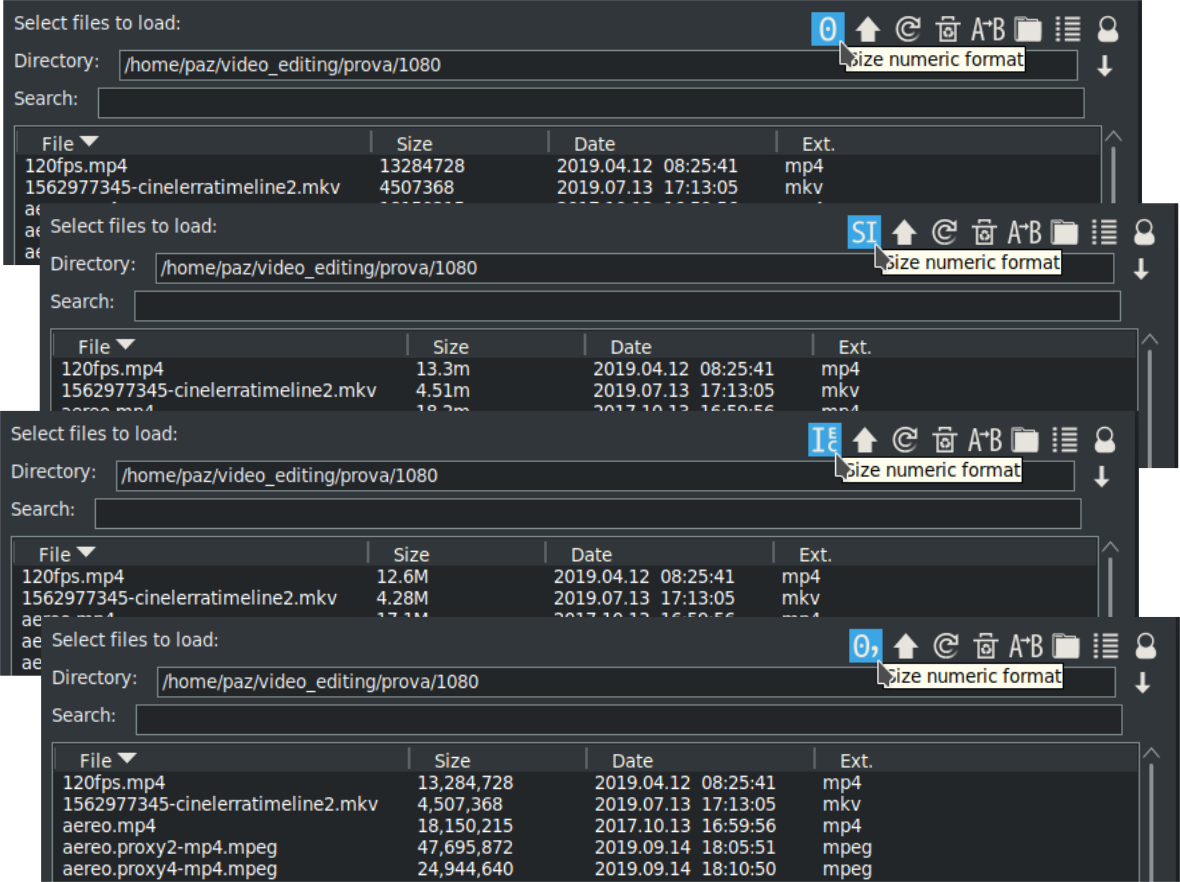
\includegraphics[width=1.0\linewidth]{load-size.png}
    \caption{Load windows with various Numeric Sizes}
    \label{fig:load-size}
\end{figure}

\subsection{Probe Order when Loading Media}%
\label{sub:probe_order_loading_media}

Why is this mentioned here?  So many programs have been written whose functionalities overlap and you may want to ensure that the one you wish to use is actually used.  Over time which one matches first may vary.  Ffmpeg is so generic that if your setting is \textit{Try ffmpeg first} it will almost certainly get used and it leaves little chance that other methods will even get a chance.  Some of the codec file drivers can open a variety of media, and some of the more common methods may have more than one file driver which could be useful to decode your media file, for example Tiff.  For expert specialized usage, when you want to guarantee that a certain method is used, you can change the \textit{probe order}.  Use the pulldown \texttt{Settings $\rightarrow$ Preferences} to get to the \textit{Interface tab} where you will see a box in the \textit{Operation} section on the left side called \textit{Probe Order}.  Click on the box and use the up/down/enabled boxes to change the order of the item you have highlighted (figure~\ref{fig:probe}).

\begin{description} [noitemsep]
    \item[Up] move the item up 1 (if the item is currently on the top, it will be moved to the bottom)
    \item[Down] move the item down 1 (similarly, if on the bottom, it will be moved to the top)
    \item[Enable] there will be a check mark if the item is currently enabled.  If you disable it, it will not be used to probe the media to determine what it is.  Double left mouse click will toggle the enabled/disabled state of the highlighted item.  If both FFMPEG Early/Late are enabled, the FFMPEG code could be run twice if the 1\textsuperscript{st} FFMPEG run failed (but so will the 2\textsuperscript{nd}!).
\end{description}

The default setup is set to duplicate the past expected behavior with the exception that CR2 for Raw Camera mode is disabled.  Changes made in the settings will be retained in the \texttt{.bcast5} file.

\begin{figure}[htpb]
    \centering
    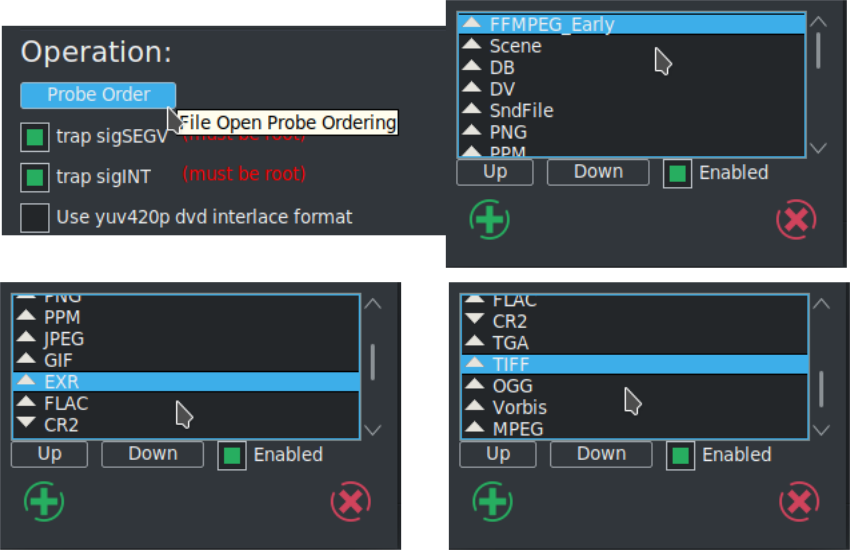
\includegraphics[width=0.8\linewidth]{probe.png}
    \caption{Three example of Probes window}
    \label{fig:probe}
\end{figure}

Figure~\ref{fig:probe} show the first few probe items.  Note that the up arrow on the left, signifies \textit{enabled}.
Scrolling down shows the next 2 pages of possible drivers for a total of 17.

The order change will not take effect until you click on the checkmark in both the Probes window and the Preferences window.  When you click on the FF button, which is in the corner of the main window (figure~\ref{fig:ff}) to change \textit{Try FFMpeg first/last}, enabling of FFMPEG\_Late or FFMPEG\_Early will be toggled automatically in Probes to match that choice but does NOT change its position in the table. Be sure to only click on the FF button without the Preference/Probes window up to avoid unexpected results.  It is also recommended to leave FFMPEG\_Early/FFMPEG\_Late close to the top/bottom positions.  There is one case where you may want to disable all of the probes if you want to force PCM -- Pulse Code Modulator.  This code is always run when all other probes fail.

\subsection{Program Selection Support after Load}%
\label{sub:program_selection_support_load}

Some kinds of media have \textit{program} streams, like captured mpeg broadcast stream data.  For example, you may be able to \textit{tune} to channel 9, but be able to see 9-1, 9-2, and 9-3 on your TV\@.  If you open a capture of this kind of media, all of the channels are present in the timeline.  To select and view just one program, you can use Alt-1 to select program 1, or Alt-2 to select program 2, etc.\ up to Alt-8.  This will remove all of the other unrelated tracks and reset the format.  This feature can be used even if there is only one program, by pressing Alt-1, and the effect will be to reset the session format to the parameters from the media probe.  Note that there may be several audio \textit{programs} associated to a video stream;
for example, there may be dialog in another language or some kind of descriptive dialog.  Since the first associated audio is always selected, this may not produce the intended results.

\begin{figure}[htpb]
    \centering
    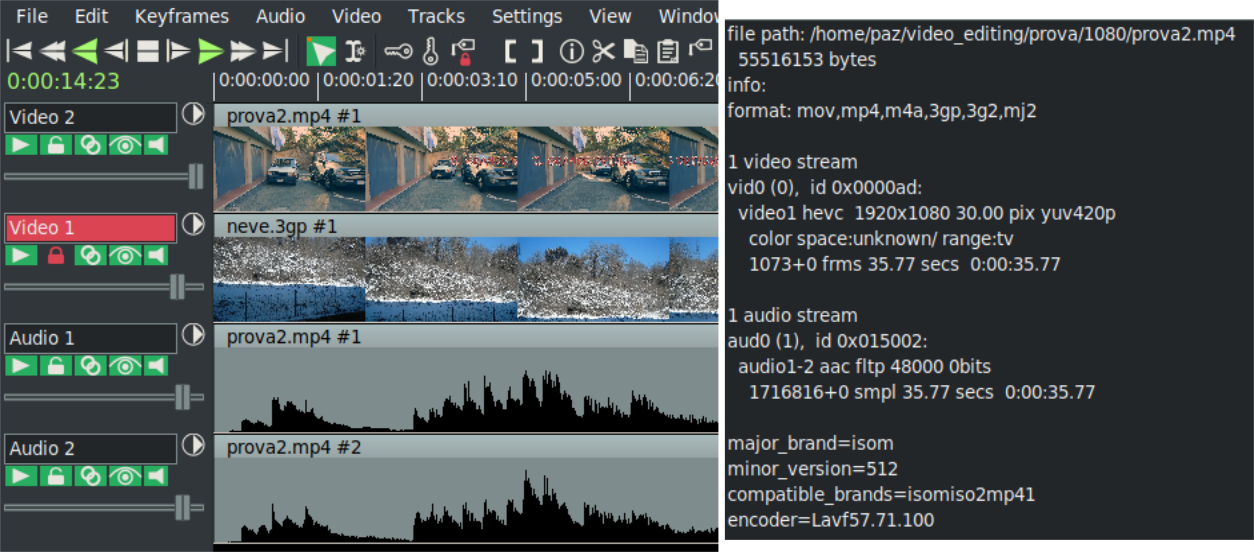
\includegraphics[width=1.0\linewidth]{stream.png}
    \caption{Multiple program streams and Asset Detail}
    \label{fig:stream}
\end{figure}

Below are screenshots illustrating multiple program streams (figure~\ref{fig:stream}).  The left screenshot is a partial main \CGG{} window showing a pre-recorded broadcast TV media/audio stream with 2 programs plus several associated audio tracks.  The second screenshot of \textit{Asset Detail} provides detailed information on each of the streams obtained through executing the \texttt{Info $\rightarrow$  Details} as explained in the section \nameref{sub:info_asset_details}.

\section{Saving Your Work}%
\label{sec:saving_your_work}

You can save your work as a project, which is what is loaded in \CGG{} now, or as an export, which is all the media it takes to reproduce your project space.

\subsection{Saving Project Files}%
\label{sub:saving_project_files}

Saving  XML files is useful to save the current state of \CGG{} before quitting an editing session. \CGG{} saves projects as XML files. There are a few options you can use to save your work via the File pulldown menu: \textit{Save}, \textit{Save as\dots}, \textit{Export project}, \textit{Save backup}.  You can either overwrite an existing file or enter a new filename. \CGG{} automatically concatenates \texttt{.xml} to the filename if no \texttt{.xml} extension is given.

When \CGG{} saves a file, it saves the EDL of the current project but does not save any media, instead just pointers to the original media files. For each media file, the XML file stores either an absolute path or just the relative path. If the media is in the same directory as the XML file, a relative path is saved. If it is in a different directory, an absolute path is saved.

You have to be careful when moving files around to avoid breaking the media linkages. You can keep the media and the XML file in the same directory forever and freely move the whole directory, since relative paths are saved. Alternatively you can save the XML file in a different directory than the media but then you can't move the media. In this case you can freely move your XML file around, since absolute paths are saved. If you saved your XML file in the same directory as your media but you would like to move location, you can change the paths from relative to absolute by going
to \texttt{File $\rightarrow$ Save as}$\dots$ and entering the new location. Similarly if you saved your project outside your media directory but you would like to move your media to another location, you can change the paths from absolute to relative by going to \texttt{File $\rightarrow$ Save as}\dots and saving your XML file in the same directory as the media.

You can also repair broken media linkage by editing the XML file in a text editor. For every media you moved, search for the old path and replace it with the new one. You should make a backup copy of your XML file before editing. You can also replace the path of every asset whose source file you moved also within the program, by entering the new location in the Asset info window. To open this window, right click on the asset in the Resources window and choose Info\dots in the popup menu. Directly type the path in the first field of the dialog or click on the magnifier on the right to browse your files. Operating
from the GUI is convenient only when a very small number of changes is needed.

Real-time effects in an XML file have to be re-created every time you play it back. The XML file also contains copies of all the source assets on disk, which takes up space.  Render your projects to a final format for more persistent storage of the output.

\subsection{Export Project – Save or Moving Project to another Computer}%
\label{sub:export_project}

\begin{figure}[htpb]
    \centering
    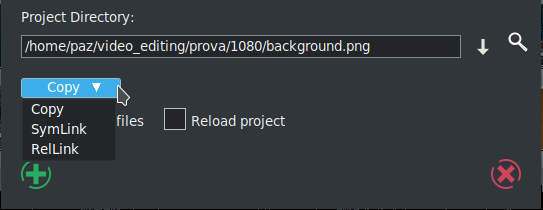
\includegraphics[width=0.6\linewidth]{export.png}
    \caption{Export Project option popup and the 3         available options.}
    \label{fig:export}
\end{figure}

A File pulldown called \textit{Export Project\dots} is also available (figure~\ref{fig:export}).  Although, it can be used in the same manner as the other \textit{save} options, it is very useful when it is necessary to move a project to another computer that may have a different top level directory structure or if you want to include subdirectories to better organize your files.  

Originally, the easiest way to maintain a project for moving to another computer, was to put all of the files in a single directory with no subdirectories along with the EDL saved \texttt{.xml} file.   This is commonly called a \textit{flat} file structure.  So if the media was in the same directory as the XML file, a relative path was saved.  If it was in a different directory, an absolute path was saved.

\noindent Definition of Fields:

\begin{description}
    \item[Project Directory] name of the directory where you want the xml file to be saved.  It will only create
    a subdirectory in 1 level of the defined directory.
    Available option types for saving a project:
    \begin{description}
        \item[Copy] all files are copied to the project directory and the xml is saved; same as original \textit{flat}.
        Option is very useful to ensure all files needed to illustrate a problem are available for analysis.
        \item[SymLink] symbolic links are created for absolute paths of media in their current location.
        \item[RelLink] symbolic links are created for relative paths of media in their current location.  This
        option allows for using relative paths without the requirement to maintain a \textit{flat} file structure
        and makes it easy to move to another computer.
    \end{description}
    \item[Overwrite files] when checked, if any files with the same name currently exist in the directory, they
    will be overwritten.  In any case, the named XML file will always be overwritten.
    \item[Reload project] when checked, after the save option the new saved project will be loaded. Default is not to do so.
\end{description}

\noindent Keep in mind that to maintain the integrity of your project xml file for easy moving to another computer, do not delete the symbolic links.  You will want to use \texttt{cp\,-a} to maintain the links for moving to a USB key or another computer.

\subsection{Information about Backups and Perpetual Session}%
\label{sub:information_backups_perpetual_session}

In an effort to minimize loss of work due to user, hardware, or software issues, \CGG{} has some automatic backup capabilities.

\CGG{} automatically saves every \textit{editing operation} to the current project on disk continuously to a file named \texttt{\$HOME/.bcast5/backup.xml}.  In the unlikely event of a crash, when you restart \CGG{}, you should select \texttt{File $\rightarrow$ Load backup} in order to continue with the operations that were recorded before the crash.  If you have more than 1 instance of \CGG{} running, only the last editing operation made in whichever instance it was last made, will overwrite the backup. 

There is still 1 more backup that may save you.  If for some reason you forgot to use \textit{Load backup}
immediately when restarting or you did a Load with \textit{Replace current project} in your current session,
you have a second chance to use \texttt{File $\rightarrow$ Load} and select \texttt{\$HOME/.bcast5/backup.prev}
as long as you only loaded a different file and have performed no editing operations.  This same file is also used by multiple instances of \CGG{}.

\textbf{Perpetual session} is very useful for working on a project over many days so you can just quit before shutting down and the next time you start up \CGG{} you will be right back where you left off.  
You will retain all of your undo’s and redo’s.  
The binary file name is \texttt{\$HOME/.bcast5/perpetual.dat} and as long as \texttt{Settings $\rightarrow$ Preferences}, the Appearance tab has the Flag \textit{Perpetual session} set this capability takes effect.  
It is very important to understand that this is not the same as the continuously editing- operation-updated \texttt{backup.xml} file.  
The perpetual.dat file is \textit{only} updated when you Quit \CGG{} in the normal manner.  
Which means if you interrupt the program, or kill it, or there is a segv or system crash, the \texttt{perpetual.dat} file will only reflect the state of your project from when you last started \CGG{}, and none of the editing/undo’s/redo’s you executed during the current session which was not ended normally.
\vspace{1ex}

Some notes to keep in mind about Perpetual session are:

\begin{itemize}
    \item when you Quit in the normal manner, it does not have to ask whether or not to save a backup
    \item takes disk space in \texttt{.bcast5} area and this could get really big
    \item after you complete a project, it is advisable to turn off the Perpetual session flag before quitting so
    that when you start a new project, you can start with a fresh perpetual.dat by turning the flag on or
    after stopping \CGG{}, delete the current \texttt{\$HOME/.bcast5/perpetual.dat} file
    \item only session data is backed up (not program feature setup)
    \item the files backup.xml and backup.prev will operate the same as before so that if there is a crash, you
    will want to use \texttt{File $\rightarrow$ Load backup} in order to continue where you were interrupted.
    \item to start \CGG{} without using your Perpetual session data even if enabled, keyin: /your\_cinelerra\_path\texttt{/bin/cin -S}
\end{itemize}


%%% Local Variables:
%%% mode: latex
%%% TeX-master: "../CinelerraGG_Manual"
%%% End:
